%************************************************
\chapter{User Guide}\label{ch:user_guide} % $\mathbb{ZNR}$
%************************************************

In this chapter ways to achieve the most common use-cases of the program will be explained. These include:

\begin{enumerate}
\item Managing (adding, deleting, editing) a stock item or bank account.
\item Placing an order.
\item Importing and exporting data.
\end{enumerate}

\section{Manage stock items and bank accounts}
\label{sec:manage_stock_item}

Upon starting the application the main window will be displayed.
The main window hosts all necessary controls for the first two use cases.

\begin{figure}[H]
\begin{center}
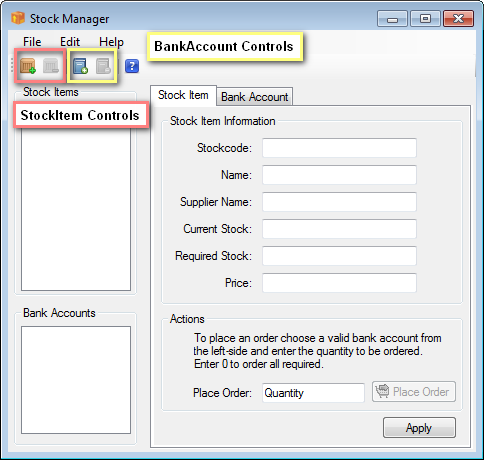
\includegraphics[width=0.8\textwidth]{gfx/main_window.png}
\caption{Main Window}
\label{fig:main_window}
\end{center}
\end{figure}

To add a stock item or a bank account a click on the appropriate button is necessary:
 
% content section
\begin{wrapfigure}{l}{5cm} % "l" or "r" for the side on the page. And the width parameter for the width of the image space.
\centering
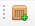
\includegraphics[scale=1]{gfx/add_stock_item.png}
\caption{Add a stock item.}
\label{fig:add_si}
\end{wrapfigure}

By clicking the icon to add a new stock item to the application, an item will be inserted into the stock item list with dummy values.

\begin{wrapfigure}{l}{5cm} % "l" or "r" for the side on the page. And the width parameter for the width of the image space.
\centering
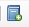
\includegraphics[scale=1]{gfx/add_bank_account.png}
\caption{Add a bank account.}
\label{fig:add_ba}
\end{wrapfigure}

By clicking the icon to add a new bank account to the application, a account will be inserted into the bank account list with dummy values.

After inserting a new stock item or bank account, the item can be chosen in the appropriate list (on the left-hand side of the application). By clicking an item, the appropriate panel will be show up, where the values can be edited.

Editing needs to be completed by clicking the \textit{apply}-button. If any incorrect values were entered, the application will inform the user about the occured mistakes.

To manage a bank account there are two more possible commands the user can issue: apart from changing the values, it is possible to deposit or withdraw money from the bank account. Therefore the user simply has to enter a number in the correct field and press the accompanying button.

\begin{figure}[H]
\begin{center}
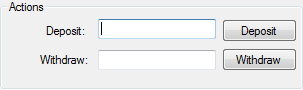
\includegraphics[scale=1.0]{gfx/bank_account_actions.png}
\caption{Depositing and withdrawing money}
\label{fig:ba_actions}
\end{center}
\end{figure}

\section{Placing an order}
\label{sec:placing_order}

\begin{wrapfigure}{l}{6cm} % "l" or "r" for the side on the page. And the width parameter for the width of the image space.
\centering
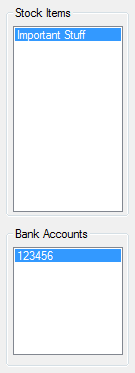
\includegraphics[scale=0.6]{gfx/highlighted_items.png}
\caption{Selection of items.}
\label{fig:highlighted_items}
\end{wrapfigure}

To place an order the user has to select a bank account and a stock item from the lists (an item needs to be highlighted in both lists).

Then a value can be entered inside the \textit{quantity}-box: either the amount of items to be ordered, or 0. By entering 0 the program will try to order the \textit{required amount}.

If enough funds are available the order will be placed and the stock information will be updated.
If not enough funds are available the application will output an error message.

\begin{figure}[H]
\begin{center}
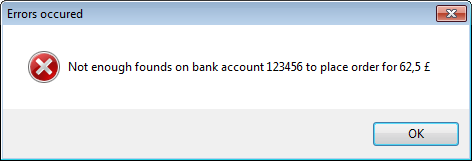
\includegraphics[scale=0.8]{gfx/not_enough_funds.png}
\caption{Placing an order without the needed funds}
\label{fig:not_enough_funds}
\end{center}
\end{figure}

\section{Importing \& exporting data}
\label{sec:import_export}

After entering stock items and bank accounts it is possible to save them to a file and open them again for later use.

Therefore the user has to choose the appropriate option from the file menu or set standard-paths and click the menu-bar icon.

\subsection{File menu}
\label{subsec:file_menu}

To save or load only one of the list the user selects \texttt{File $\Rightarrow$ Save (Open) $\Rightarrow$ Save (Open) bank accounts / Save (Open) stock items}.

\begin{figure}[H]
\begin{center}
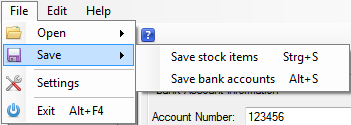
\includegraphics[scale=0.8]{gfx/save_file_menu.png}
\caption{Saving via file menu}
\label{fig:save_file_menu}
\end{center}
\end{figure}

\subsection{Menu-bar icon}

To save via the menu icon it is necessary to first set default file paths for the files \footnote{As soon as these paths are set, the application will also attempt to load items and bank account on start-up.}. The paths can be set in the \texttt{settings window} found under \texttt{File $\Rightarrow$ Settings}.

\begin{figure}[H]
\begin{center}
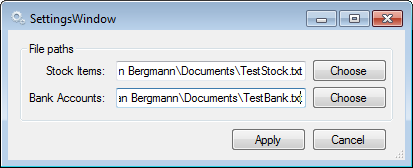
\includegraphics[scale=0.8]{gfx/settings_window.png}
\caption{Settings window}
\label{fig:settings_window}
\end{center}
\end{figure}

After setting these paths both lists can be saved with a single click on the menu-bar icon (denoted by two disks).
